% Header trang
\noindent
{\fontsize{9}{11}\selectfont\bfseries 290}\qquad
{\fontsize{8.5}{11}\selectfont\sffamily\bfseries CHƯƠNG 4}\quad
{\fontsize{8.5}{11}\selectfont\sffamily Các ứng dụng của đạo hàm}
\vspace{6pt}

% Phần dự án ứng dụng phía trên (Applied Project: Cầu vồng)
\noindent
\begin{tcolorbox}[
  enhanced,
  colback=projectbg,
  colframe=projectbg,
  boxrule=0pt,
  arc=0pt,
  left=8pt, right=8pt, top=8pt, bottom=8pt
]
  \begin{minipage}[t]{48mm}
    \vspace{0pt}
    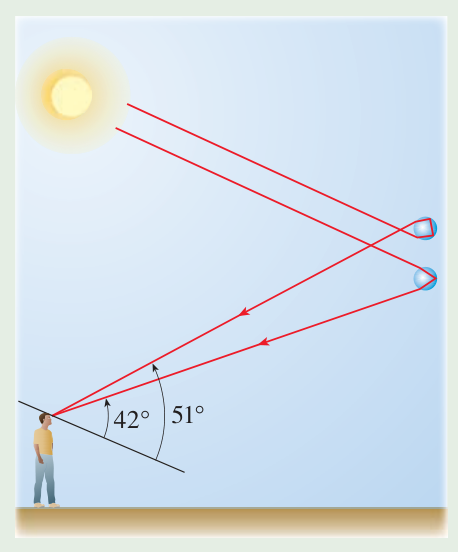
\includegraphics[width=\linewidth, keepaspectratio]{images/p0325_fig1.png}
  \end{minipage}%
  \hspace{7mm}%
  \begin{minipage}[t]{125mm}
    \vspace{0pt}
    {\fontsize{9}{12}\selectfont
    Lấy $k = \frac{4}{3}$, hãy chứng minh rằng độ lệch nhỏ nhất vào khoảng $129^\circ$ và do đó góc cầu vồng đối với cầu vồng thứ cấp vào khoảng $51^\circ$, như chỉ ra trong hình bên trái.

    \vspace{5pt}
    \textbf{4.} Hãy chứng minh rằng các màu sắc trong cầu vồng thứ cấp xuất hiện theo thứ tự ngược lại so với cầu vồng sơ cấp.
    }

    \vspace{6pt}
    \begin{minipage}{\linewidth}
      \begin{tabular}{@{}c@{\hspace{3pt}}l@{}}
        \rotatebox{90}{\fontsize{5}{6}\selectfont\color{black!60} Leonid Andronov / Shutterstock.com} &
        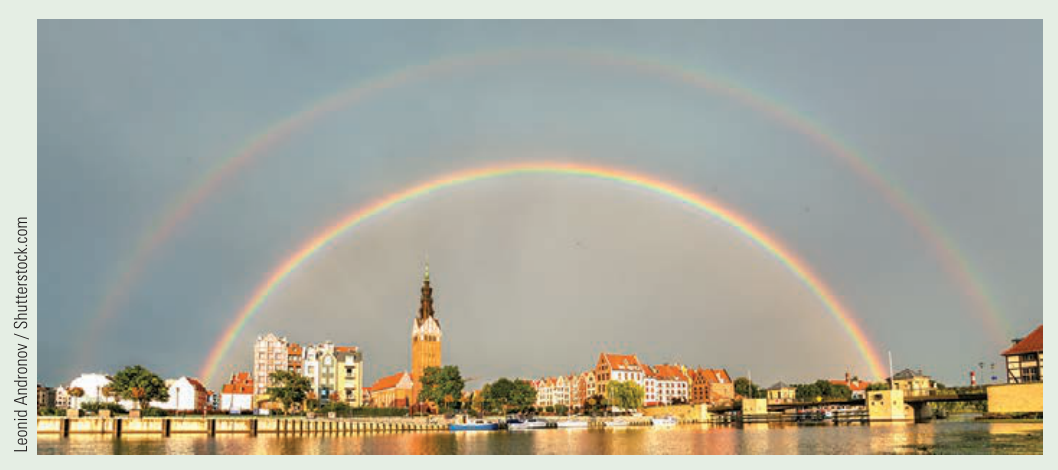
\includegraphics[width=0.96\linewidth]{images/p0325_fig2.png}
      \end{tabular}
    \end{minipage}
  \end{minipage}
\end{tcolorbox}

\vspace{10pt}

% Tiêu đề mục 4.2: Định lý giá trị trung bình
\noindent
\begin{minipage}[c]{48mm}
  \raggedleft
  \begin{minipage}[c]{16mm}
    \color{stewartblue}
    \rule{\linewidth}{1pt}\\[2.5pt]
    \rule{\linewidth}{1pt}\\[2.5pt]
    \rule{\linewidth}{1pt}
  \end{minipage}%
  \hspace{6pt}%
  {\fontsize{24}{24}\selectfont\sffamily\bfseries\color{stewartblue} 4.2}
\end{minipage}%
\hspace{3.5mm}%
{\color{stewartblue}\rule[-6pt]{1.2pt}{25pt}}%
\hspace{3.5mm}%
\begin{minipage}[c]{125mm}
  {\fontsize{18}{22}\selectfont\sffamily\bfseries\color{stewartblue} Định lý giá trị trung bình}
\end{minipage}

\vspace{10pt}

% Nội dung dẫn nhập trước Định lý Rolle
\noindent
\begin{minipage}[t]{48mm}
  % Khoảng trống tương ứng với lề trái
\end{minipage}%
\hspace{7mm}%
\begin{minipage}[t]{125mm}
  {\fontsize{9.5}{13.5}\selectfont
  Chúng ta sẽ thấy rằng nhiều kết quả trong chương này phụ thuộc vào một sự thật trung tâm, được gọi là \textit{Định lý giá trị trung bình}.

  \vspace{8pt}
  {\color{stewartblue}$\blacksquare$}\;\; {\sffamily\bfseries Định lý Rolle}

  \vspace{3pt}
  Để đi đến Định lý giá trị trung bình, trước tiên chúng ta cần kết quả sau đây.
  }
\end{minipage}

\vspace{8pt}

% Khung ghi chú Rolle ở lề trái và Khung Định lý Rolle ở cột chính
\noindent
\begin{minipage}[t]{48mm}
  \vspace{0pt}
  \begin{tcolorbox}[
    enhanced,
    colback=white,
    colframe=rolleboxgreen,
    boxrule=0.7pt,
    arc=2pt,
    left=5pt, right=5pt, top=5pt, bottom=5pt
  ]
    {\sffamily\bfseries\color{rolleboxgreen} Rolle}\par\vspace{3pt}
    {\fontsize{8}{10.5}\selectfont
    Định lý Rolle được công bố lần đầu tiên vào năm 1691 bởi nhà toán học người Pháp Michel Rolle (1652--1719) trong một cuốn sách có tựa đề \textit{Méthode pour resoudre les egalitez}. Ông từng là một người chỉ trích kịch liệt các phương pháp trong thời đại của mình và công kích giải tích là một “tập hợp những ngụy biện khéo léo”. Tuy nhiên, về sau ông đã bị thuyết phục về tính đúng đắn bản chất của các phương pháp giải tích.\par}
  \end{tcolorbox}
\end{minipage}%
\hspace{7mm}%
\begin{minipage}[t]{125mm}
  \vspace{0pt}
  \begin{tcolorbox}[
    enhanced,
    colback=white,
    colframe=theoremred,
    boxrule=0.8pt,
    arc=0pt,
    left=9pt, right=9pt, top=7pt, bottom=7pt
  ]
    {\sffamily\bfseries\color{theoremred} Định lý Rolle}\quad
    {\fontsize{9.5}{13.5}\selectfont Giả sử $f$ là một hàm số thỏa mãn ba giả thiết sau:}
    \begin{enumerate}[label=\textbf{\arabic*.}, leftmargin=18pt, itemsep=2pt, topsep=3pt, parsep=0pt]
      \item $f$ liên tục trên đoạn đóng $[a, b]$.
      \item $f$ khả vi trên khoảng mở $(a, b)$.
      \item $f(a) = f(b)$
    \end{enumerate}
    \vspace{2pt}
    {\fontsize{9.5}{13.5}\selectfont Khi đó tồn tại một số $c$ trong khoảng $(a, b)$ sao cho $f'(c) = 0$.}
  \end{tcolorbox}

  \vspace{6pt}
  {\fontsize{9.5}{13.5}\selectfont
  Trước khi đưa ra chứng minh, chúng ta hãy xem xét đồ thị của một số hàm số điển hình thỏa mãn ba giả thiết trên. Hình 1 thể hiện đồ thị của bốn hàm số như vậy. Trong mỗi trường hợp, dường như có ít nhất một điểm $(c, f(c))$ trên đồ thị mà tại đó tiếp tuyến nằm ngang và do đó $f'(c) = 0$. Như vậy, Định lý Rolle là hoàn toàn hợp lý.
  }
\end{minipage}

\vspace{10pt}

% Hình 1 (Cụm 4 đồ thị trải ngang trang)
\noindent
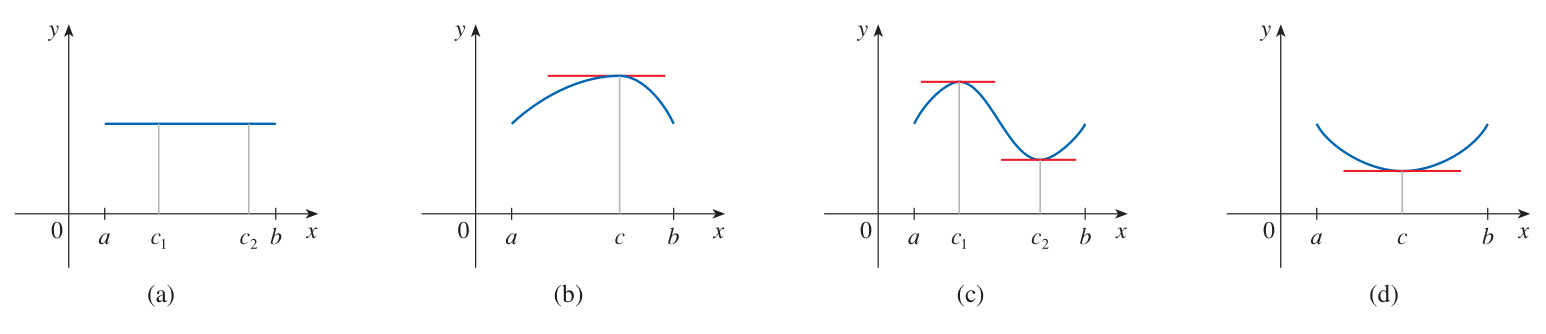
\includegraphics[width=\textwidth]{images/p0325_fig3.png}

\vspace{3pt}
\noindent
\begin{minipage}[t]{48mm}
  {\sffamily\bfseries\small HÌNH 1}
\end{minipage}

% Footer bản quyền
\vfill
\begin{center}
  {\fontsize{5.5}{7}\selectfont\color{black!60}
  Copyright 2021 Cengage Learning. All Rights Reserved. May not be copied, scanned, or duplicated, in whole or in part. WCN 02-200-203\\[1pt]
  Due to electronic rights, some third party content may be suppressed from the eBook and/or eChapter(s). Editorial review has deemed that any suppressed content does not materially affect the overall learning experience. Cengage Learning reserves the right to remove additional content at any time if subsequent rights restrictions require it.\par}
\end{center}
